\chapter{Experimental Results and Analysis}

In analysis of a process, experiments are commonly used to evaluate the inputs to the process which most times define the output of the process. They also help pinpoint the appropriate and thus target inputs to achieve a desired result. The output of the video summarizer is compared with the expected output to verify the correctness of the system. There are several metrics for comparison. Analyzing the experimental output is verifying whether the evaluation metrics are satisfied. This chapter discusses the performance characteristics of the system.

\section{Evaluation Metric}

Evaluation metrics are the criteria for testing different algorithms. The behavior of the algorithms or techniques can be determined using these metrics. In this project, we do not have many concrete objective methods for testing the summary, and some metrics that we have are subjective as well. The outputs that are obtained from the different inputs given to the summarizer are compared with the expected output to check whether the metrics are satisfied.

\section{Experimental Dataset}

We collected sample video clips in different urban areas with sparse motion and activity, with only 1-2 events occurring once every few seconds. These clips were used for developing and testing the algorithm.

\begin{figure}[H]
    \centering
    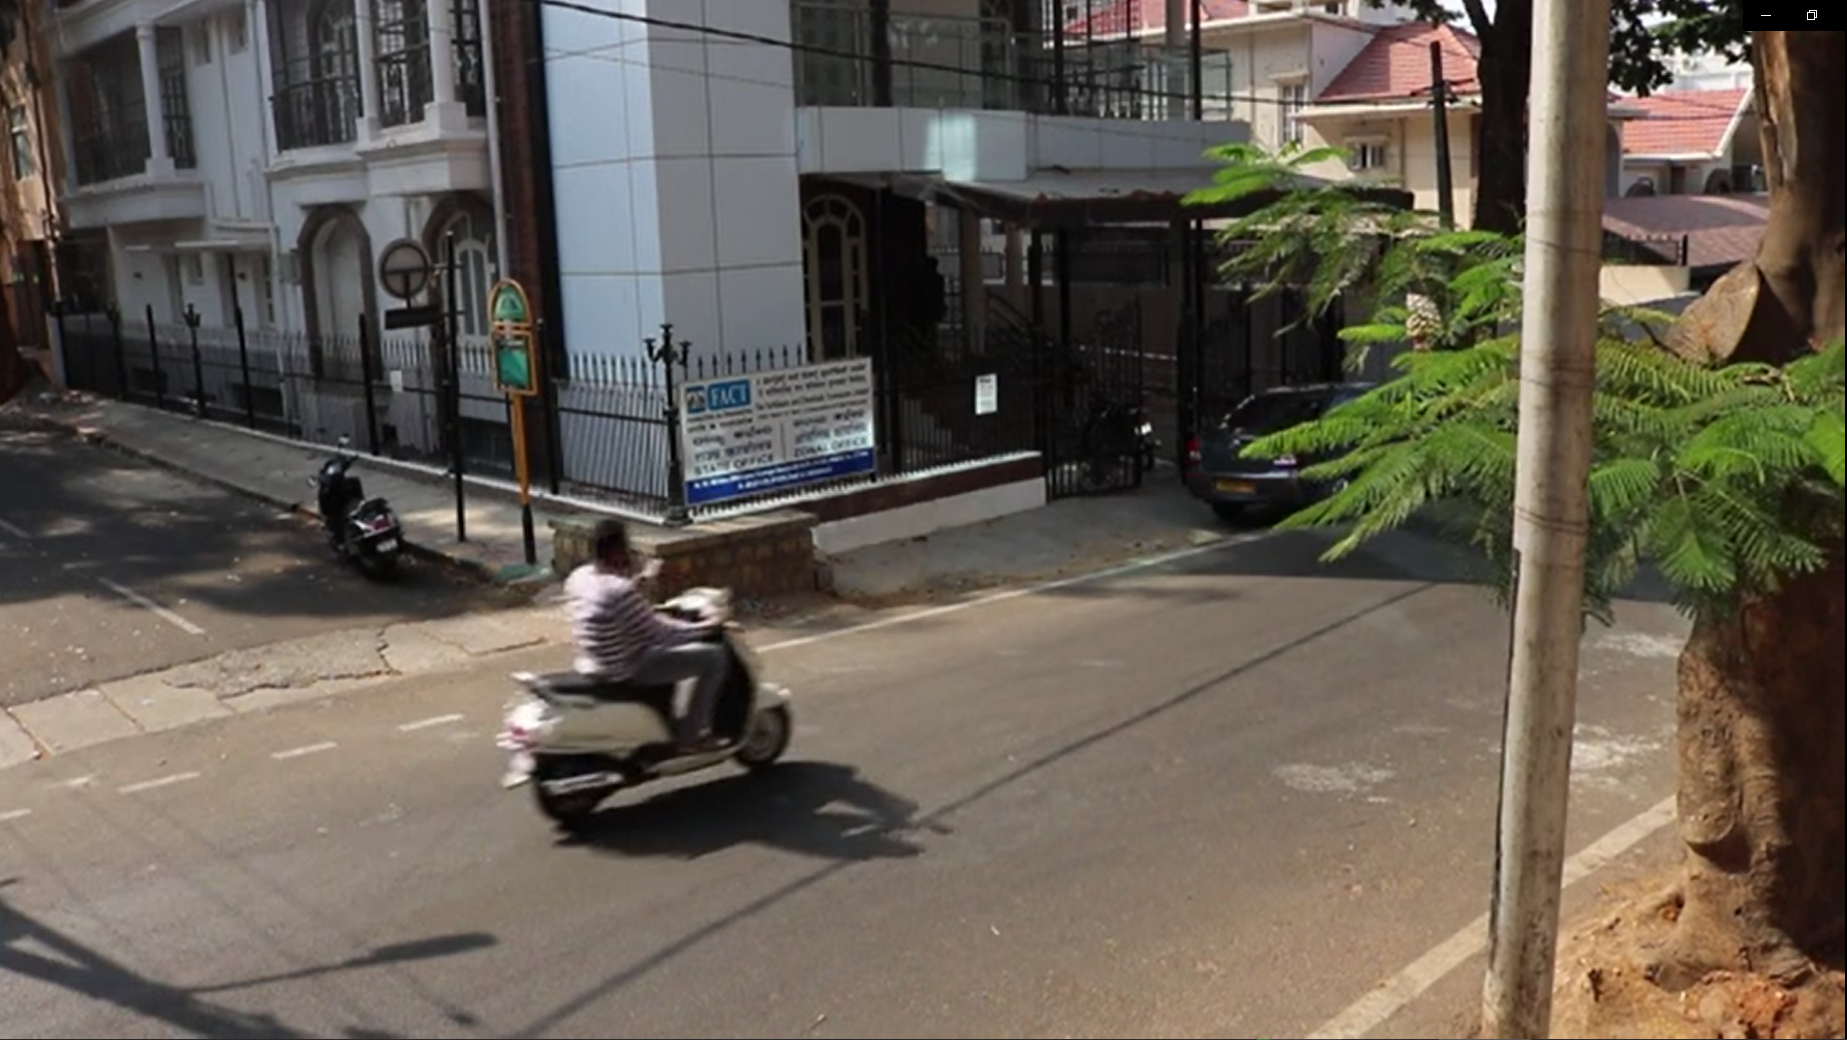
\includegraphics[scale=0.3]{sample-frame.png}
    \caption{Image from one of the test clips, with just a single bike moving in the frame}
    \label{img:sample-frame}
\end{figure}

\section{Performace Analysis}

This section explains the experimental results of this project. The system performance was satisfactory and was mostly successful with the tested input clips, with some limitations which will be mentioned in the further sections.

    \subsection{Objective Evaluation Parameters}

    \begin{itemize}
        \item \textbf{Exhaustiveness of summary}
        The summarizer must retain all the events that occurred or the events of the specified type in the tag-based summary generation. \\
        Result: All significant events are selected in the events
        \item \textbf{Compression factor}
        Given by Length of original input/Length of summary. The compression factor must be as high as possible while keeping the overlap factor to a minimum. \\
        Result: There is a compression factor of 4-5x for our sample videos
        \item \textbf{Overlap factor}
        A number between 0 and 1 which indicates the amount of overlapping (intersection) between the tubes in the summary video. 0 indicates no overlap and 1 indicates complete overlap of every clip. \\
        Result: All videos have overlap lower than 0.1
    \end{itemize}

    \subsection{Subjective Evaluation Parameters}

    \begin{itemize}
        \item \textbf{Semantic structure of events}
        Interacting events (that occur in the same time and space) must be shown together. \\
        Result: All the interacting events are always shown together
        \item \textbf{Realistic appearance}
        The events must be extracted and be blended into the background seamlesslyand appear realistic. \\
        Result: Realistic appearance in most cases, with some halo around object when at the edges of the frame, or when there is intersection.
    \end{itemize}


\section{Summary}

The video summary method we have developed performs in real-time (30fps) for the real-time phase and runs reasonably fast in the query phase as well. It takes about 1 min about 1 minute for generating a summary video of 10-15 secs. The outputs are acceptable for the regular summarization (with all events) and the tag-based summarization, except a few cases where small or fast-moving objects are not detected. The optimization and blending process can be improved further to ensure that overlap is further reduced.
